\documentclass{article}
\usepackage[utf8]{inputenc}
\usepackage{graphicx}
\usepackage{amsmath, amssymb}
\usepackage[left=3cm,right=3cm,top=2cm,bottom=2cm]{geometry}
\usepackage{url}
\usepackage{cite}
\usepackage{graphicx}
\usepackage{tabto}


\usepackage{hyperref}
\hypersetup{
    colorlinks,
    citecolor=black,
    filecolor=black,
    linkcolor=black,
    urlcolor=black
}
\begin{document}

\begin{titlepage}
    \begin{center}
        \vspace*{6cm}
 
        \textbf{\huge{Projet traitement de l'information}}
 
        \vspace{0.5cm}
        \large{\'Etude des campagnes Kickstarter et de leur r\'eussite}
             
        \vspace{1.5cm}
 
        \textbf{Rodrigez Esteban, Coutan Thomas, Beno\^\i t Ch\'enard}
 
        \vfill
        Informatique\\
        ENSEIRB-MATMECA\\
        2022-2023 
    \end{center}
 \end{titlepage}

\renewcommand\contentsname{Table des mati\`eres}
\tableofcontents
\newpage

\section{Introduction}

\tabto{1cm} Dans ce rapport, nous étudierons les projets Kickstarters et essaierons de trouver des facteurs de réussite. Nous analyserons mais aussi quantitatives.
Pour cela, nous utiliserons différentes méthodes pour traiter les données, notamment des régressions linéaires pour déterminer quelles catégories sont les plus prolifiques ou encore quel monnaie (et donc quel pays) est la plus donnée par donateurs.
\tabto{1cm} Nous expliquerons plus précisemment dans la section \ref{donnees} la base de données que nous allons utiliser, dans la section \ref{methode}, nous détaillerons la méthode avec laquelle nous avons traité ces données.
Ensuite, dans la section \ref{analyse}, nous analyserons les différents résultats obtenus. Enfin, nous concluerons en section \ref{Conclusion}. 

\section{Présentation des données}
\label{donnees}
\tabto{1cm} Les données sur lesquelles nous allons travailler sont des données nous donnant diverses informations sur des projets Kickstarter. Kickstarter est une plateforme de financement partifcipatif qui permet à de noumbreux indépendants de récolter des fonds pour développer 
leur projet. Ainsi, des projets comme le jeu Star Citizen ou la montre Pebble Time ont pu voir le jour grâce au soutien des donateurs. Les données nous donnent comme information la catégorie, l'objectif initial, le nombre de donateurs et le montant levé au total. Nous avons aussi les dates de début et de fin de la campagne.
Aussi, nous avons des informations sur les devises(monnaie) et pays d'origine de ces campagnes.

\section{Présentation de la méthode}
\label{methode}
\tabto{1cm} Nous avons décidé d'étudier plusieurs points: les catégories qui rapportent le plus d'argent par donateur, le montant donnée par donateur en fonction de la devise et enfin de voir si les campagnes remplissent généralement leur objectif initial.
\tabto{1cm}Pour les deux premiers points, nous utiliserons des régressions linéaires. 
\tabto{1cm} Pour le troisième, nous réprésenteront les campagnes dans un espace en 3 dimensions avec commes axes: le montant récolté, l'objectif et le nombre de donateurs.
\section{Analyse des résultats}
\label{analyse}

\subsection{Montant donné par donateur en fonction de la catégorie}
\label{devise}
Nous pouvons observer sur la figure \ref{fig_categorie} que c'est bien.

\begin{figure}[htbp]
    \graphicspath{{graph/}} 
    \centerline{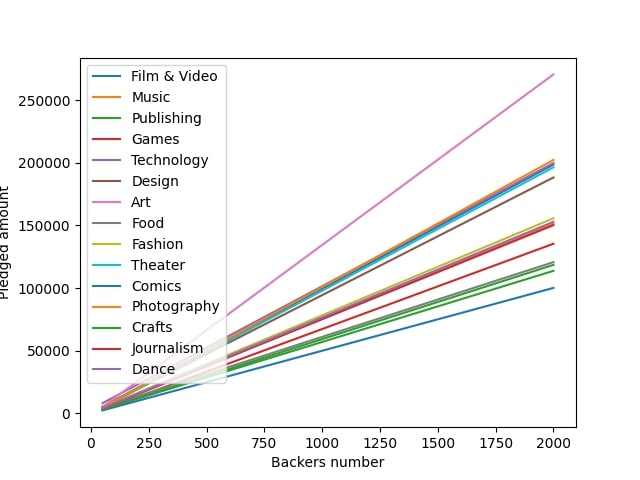
\includegraphics[scale=0.4]{main_category.jpg}}
    \caption{Montant donné en fonction du nombre de donateurs et de la devise}
    \label{fig_categorie}
\end{figure}    
\newpage 

\subsection{Montant donné par donateur en fonction de la devise}
\label{categorie}
\tabto{1cm} Nous pouvons observer sur la figure \ref{fig_devise} un graphique représentant le montant total récolté (en équivalent US dollar) en fonction de la devise et du nombre de donateurs. 
Ainsi notre régression linéaire nous permet de déterminer la moyenne du montant des contributions par devise. En effet, cette moyenne est égale à la pente des droites. Ainsi, on voit se distinguer 3 devises dont le montant moyen des contributions est plus élevé: 
le Dollar de Honk Kong, la couronne danoise et la couronne norvégienne. Au contraire, la livre sterling est la monnaie dont les contributions sont en moyenne les plus faibles.

\begin{figure}[htbp]
    \graphicspath{{graph/}} 
    \centerline{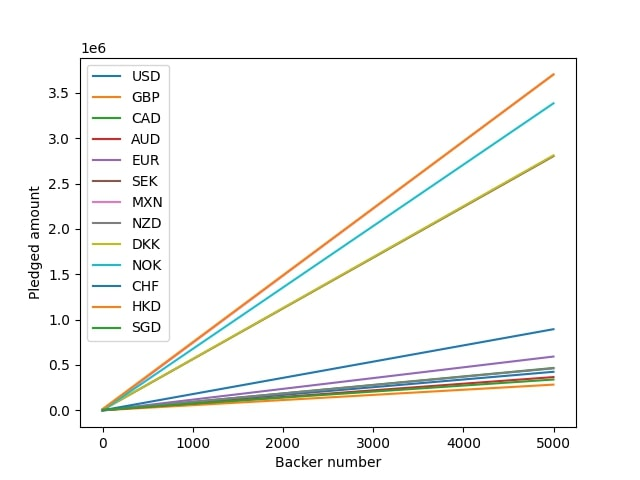
\includegraphics[scale=0.4]{currency_comparison.jpg}}
    \caption{Montant donné en fonction du nombre de donateurs et de la catégorie}
    \label{fig_devise}
\end{figure}

\newpage

\subsection{Réussite des campagnes}
\label{reussite}
\tabto{1cm} Nous pouvons observer sur la figure \ref{fig_reussite} qu'il y a énormément de campagnes qui se situent dans le coin en bas à gauche, c'est-à-dire que la plupart récolte pas énormément d'argent et mobilisent peu de donateurs.
Cependant, une partie non négligeable des campagnes parviennent à dépasser leur objectif, il y a aussi des "anomalies", notamment une campagne qui n'a pas beaucoup de donateurs et un objectif initial peu élevé mais qui a tout de même récolté énormément d'argent.

\begin{figure}[htbp]
    \graphicspath{{graph/}} 
    \centerline{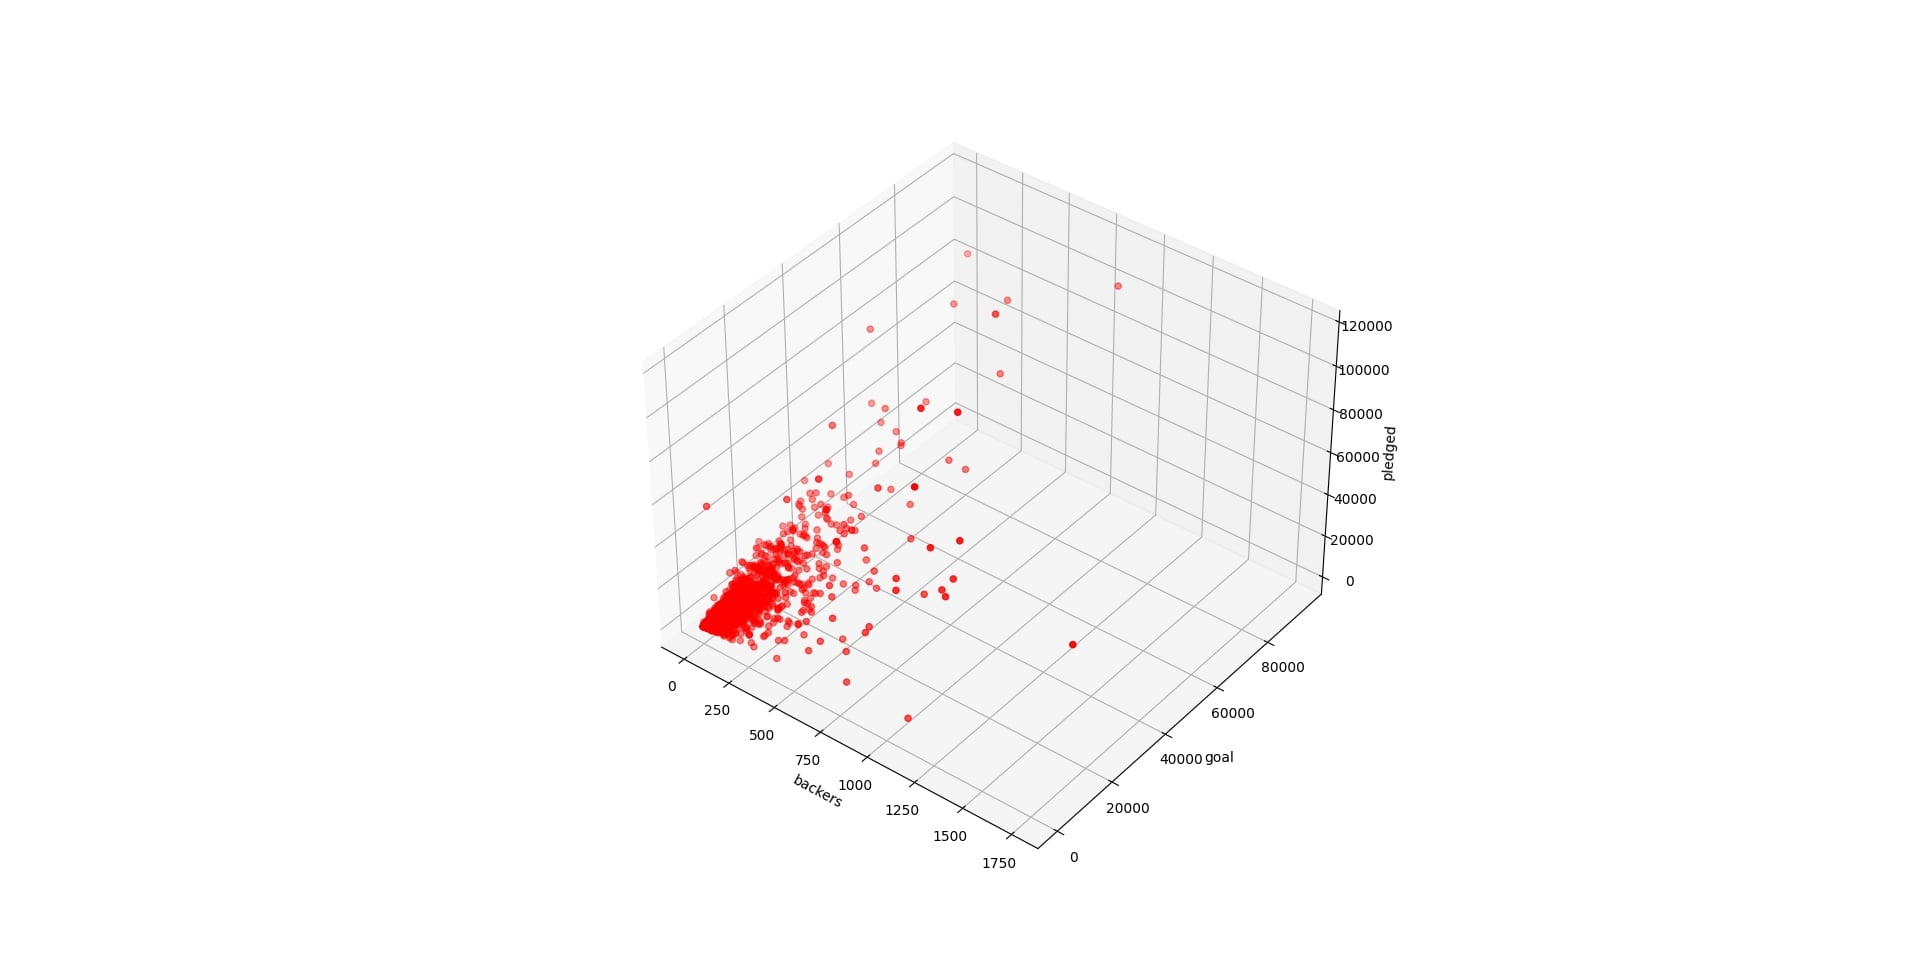
\includegraphics[scale=0.3]{goal_pledged_backers.jpg}}
    \caption{Réprésentation dans l'espace des campganes Kickstarter}
    \label{fig_reussite}
\end{figure}

\newpage

\section{Conclusion}
\label{Conclusion}
\tabto{1cm} En somme, nous avons réussi déterminer les catégories dans lesquelles les donateurs donnent le plus mais aussi quel devise sont les plus généreusement donnée (par utillisateur). Ces deux points peuvent nous permettre, grâce aux régressions linéaires de prévoir le montant moyen que les donateurs vont 
donner en fonction de la catégorie et de la devise de la campagne. Nous pensons qu'une étude sur la duréee des campagnes pourrait aussi être utile afin de trouver tous les paramètres les plus optimisés pour réussir sa campagne. 

\end{document}